% Options for packages loaded elsewhere
\PassOptionsToPackage{unicode}{hyperref}
\PassOptionsToPackage{hyphens}{url}
%
\documentclass[
]{book}
\usepackage{amsmath,amssymb}
\usepackage{iftex}
\ifPDFTeX
  \usepackage[T1]{fontenc}
  \usepackage[utf8]{inputenc}
  \usepackage{textcomp} % provide euro and other symbols
\else % if luatex or xetex
  \usepackage{unicode-math} % this also loads fontspec
  \defaultfontfeatures{Scale=MatchLowercase}
  \defaultfontfeatures[\rmfamily]{Ligatures=TeX,Scale=1}
\fi
\usepackage{lmodern}
\ifPDFTeX\else
  % xetex/luatex font selection
\fi
% Use upquote if available, for straight quotes in verbatim environments
\IfFileExists{upquote.sty}{\usepackage{upquote}}{}
\IfFileExists{microtype.sty}{% use microtype if available
  \usepackage[]{microtype}
  \UseMicrotypeSet[protrusion]{basicmath} % disable protrusion for tt fonts
}{}
\makeatletter
\@ifundefined{KOMAClassName}{% if non-KOMA class
  \IfFileExists{parskip.sty}{%
    \usepackage{parskip}
  }{% else
    \setlength{\parindent}{0pt}
    \setlength{\parskip}{6pt plus 2pt minus 1pt}}
}{% if KOMA class
  \KOMAoptions{parskip=half}}
\makeatother
\usepackage{xcolor}
\usepackage{longtable,booktabs,array}
\usepackage{calc} % for calculating minipage widths
% Correct order of tables after \paragraph or \subparagraph
\usepackage{etoolbox}
\makeatletter
\patchcmd\longtable{\par}{\if@noskipsec\mbox{}\fi\par}{}{}
\makeatother
% Allow footnotes in longtable head/foot
\IfFileExists{footnotehyper.sty}{\usepackage{footnotehyper}}{\usepackage{footnote}}
\makesavenoteenv{longtable}
\usepackage{graphicx}
\makeatletter
\def\maxwidth{\ifdim\Gin@nat@width>\linewidth\linewidth\else\Gin@nat@width\fi}
\def\maxheight{\ifdim\Gin@nat@height>\textheight\textheight\else\Gin@nat@height\fi}
\makeatother
% Scale images if necessary, so that they will not overflow the page
% margins by default, and it is still possible to overwrite the defaults
% using explicit options in \includegraphics[width, height, ...]{}
\setkeys{Gin}{width=\maxwidth,height=\maxheight,keepaspectratio}
% Set default figure placement to htbp
\makeatletter
\def\fps@figure{htbp}
\makeatother
\setlength{\emergencystretch}{3em} % prevent overfull lines
\providecommand{\tightlist}{%
  \setlength{\itemsep}{0pt}\setlength{\parskip}{0pt}}
\setcounter{secnumdepth}{5}
\usepackage{booktabs}
\ifLuaTeX
  \usepackage{selnolig}  % disable illegal ligatures
\fi
\usepackage[]{natbib}
\bibliographystyle{plainnat}
\IfFileExists{bookmark.sty}{\usepackage{bookmark}}{\usepackage{hyperref}}
\IfFileExists{xurl.sty}{\usepackage{xurl}}{} % add URL line breaks if available
\urlstyle{same}
\hypersetup{
  pdftitle={Finheim's Guide to Long Term Investing in Stocks},
  pdfauthor={João Montanher},
  hidelinks,
  pdfcreator={LaTeX via pandoc}}

\title{Finheim's Guide to Long Term Investing in Stocks}
\author{João Montanher}
\date{2024-06-25}

\begin{document}
\maketitle

{
\setcounter{tocdepth}{1}
\tableofcontents
}
\hypertarget{introduction}{%
\chapter{Introduction}\label{introduction}}

This book has been written, coded and compiled with the aim of making life easier for the long-term stock investor, as it is easy to get lost in the vast amount of data that countless companies listed on the stock exchanges generate.

Given this problem, I decided to explore the daily stock prices and fundamental data of companies with the aim of looking for profitable and financially healthy companies (although nothing written in this book is an investment recommendation).

As the financial market is in constant flux, this book will be too, which is why I'll be updating this book quite frequently and selected GitHub as the mean of publishing (in programmers' parlance: ``committing'') it.

I've divided this book into two parts:

\textbf{Fundamentals}, where I explain the fundamentals behind the graphs plotted in this book (I recommend bookmarking this page in some way, as you'll want to return to it often).

\textbf{List of Companies}, which have demonstrated good financial health and positive profitability (once again I reiterate: this book does not work with company recommendations).

If you want to contribute with the project, you can modify and/or improve the source code of the book in \href{https://github.com/JoaoMontanher/Finheim-Main-Book}{Github}. Also, you can share and discuss ideas for the project in our \href{https://www.reddit.com/r/Finheim/}{Reddit} group.

Another thing: When I say ``Long-term investment'', I mean holding a company in your portfolio for years, not trading methods that promise miraculous high returns in the short term.

\hypertarget{fundamentals}{%
\chapter{Fundamentals}\label{fundamentals}}

The \textbf{Internal Rate of Return (IRR)} is a way of calculating the profitability of an investment considering contributions and sales of assets of various amounts (in this case, the sale only takes place at the end, and the contributions have constant values more the dividends distributed). We can interpret the \textbf{IRR} as an application of compound interest at more complex situations. In our case, the lump sum contributions plus dividends were calculated for a period of 10 years (or 5 years for newer companies on the stock exchange).

\textbf{Net Income/Loss} represents the company's profitability after deducting all general, financial, depreciation and tax expenses. A company considered profitable for us is a company with increasing profits over the years.

In accounting, \textbf{Research and Development} are considered expenses, but for us, it is considered an investment.

When the annual ``Expenses'' of \textbf{R\&D} increases, it means that the company is active with innovation and we could expect surprises for the future of the company and a possible increase of the Net income.

The balance sheet of a company financially represents everything that is used in the operation of the company alongside all its financial obligations. To do this, the balance sheet is divided into three main parts: assets, liabilities and shareholders' equity.

Below is a simplified example of a balance sheet:

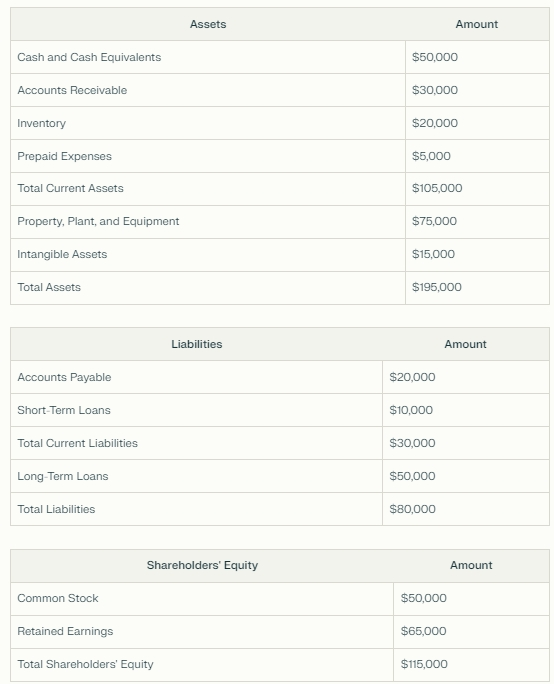
\includegraphics{BalanceSheet.jpg}

Assets are all the company's property and rights, such as machinery and cash on hand, whether obtained with third-party capital (Liabilities) or owners' capital (Equity).

Liabilities represent all the company's financial obligations to third parties, such as debts and accounts payable.

If we subtract the assets from the total liabilities, we get the shareholders' equity, which consists mainly of the company's share capital. So, mathematically: Assets = Liabilities + Equity.

If we divide equity by total assets, we find the \textbf{Equity Ratio}, a metric that shows the proportion of total assets that is financed by shareholders' capital. The higher this metric, the less the company depends on third-party capital and/or debt.

We can also divide assets and liabilities into current (or short-term) assets and liabilities. If we divide current assets by current liabilities, we get the \textbf{Current Ratio}, which shows the company's ability to pay its short-term obligations with its short-term assets.

\hypertarget{companies}{%
\chapter{Companies}\label{companies}}

\hypertarget{nvda}{%
\section{NVDA}\label{nvda}}

NVIDIA (NVDA), a leading American technology company, creates graphics processing units (GPUs) that power high-performance computing and gaming, along with developing artificial intelligence hardware and software and designing chips for various markets like mobile and automotive industries.

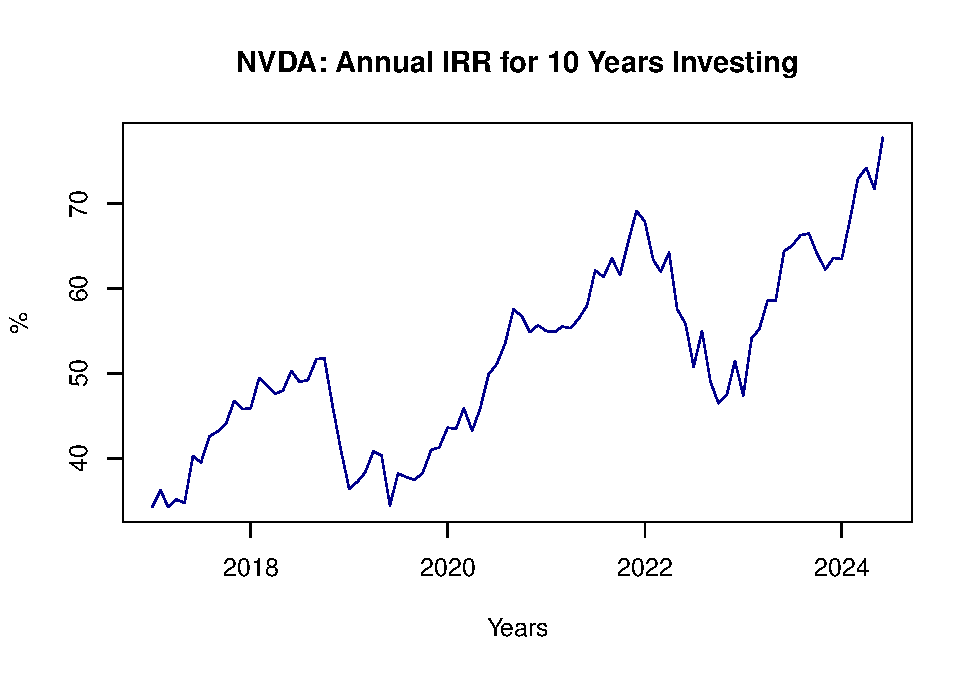
\includegraphics{_main_files/figure-latex/unnamed-chunk-1-1.pdf}
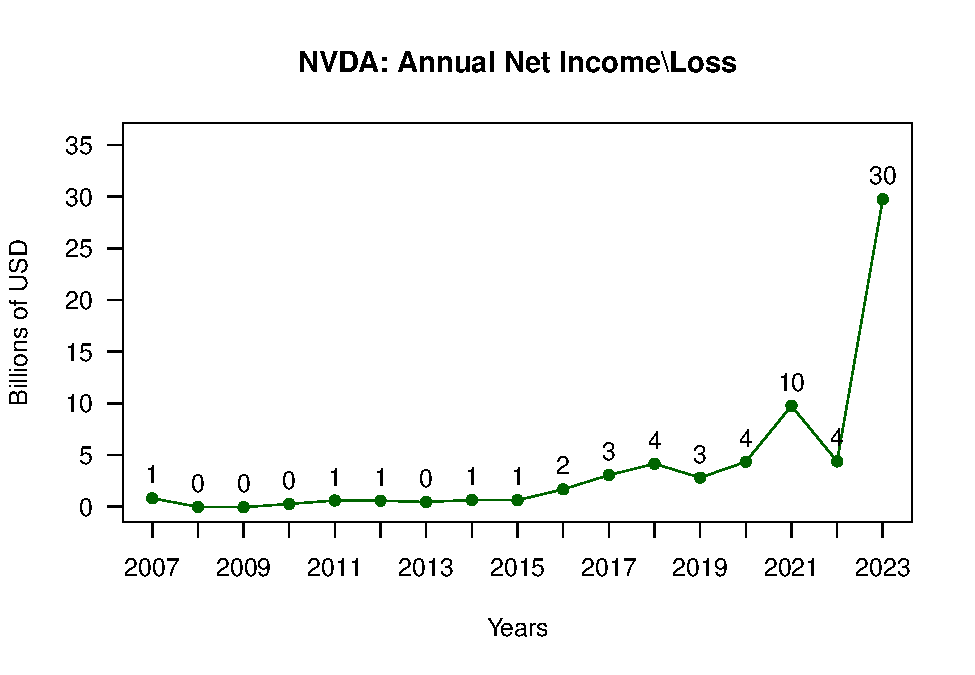
\includegraphics{_main_files/figure-latex/unnamed-chunk-1-2.pdf}
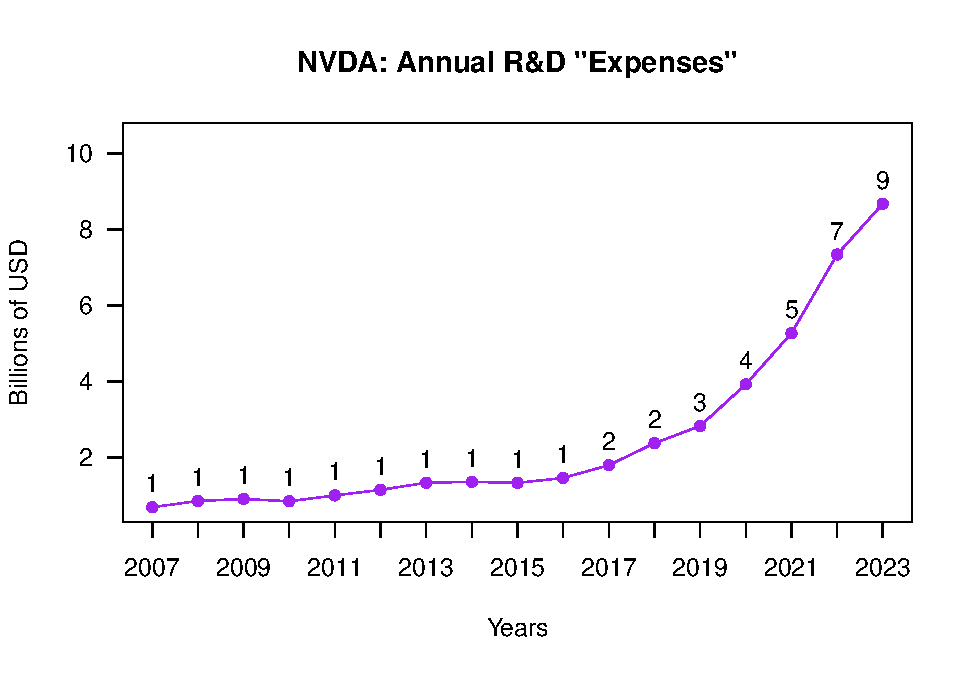
\includegraphics{_main_files/figure-latex/unnamed-chunk-1-3.pdf}
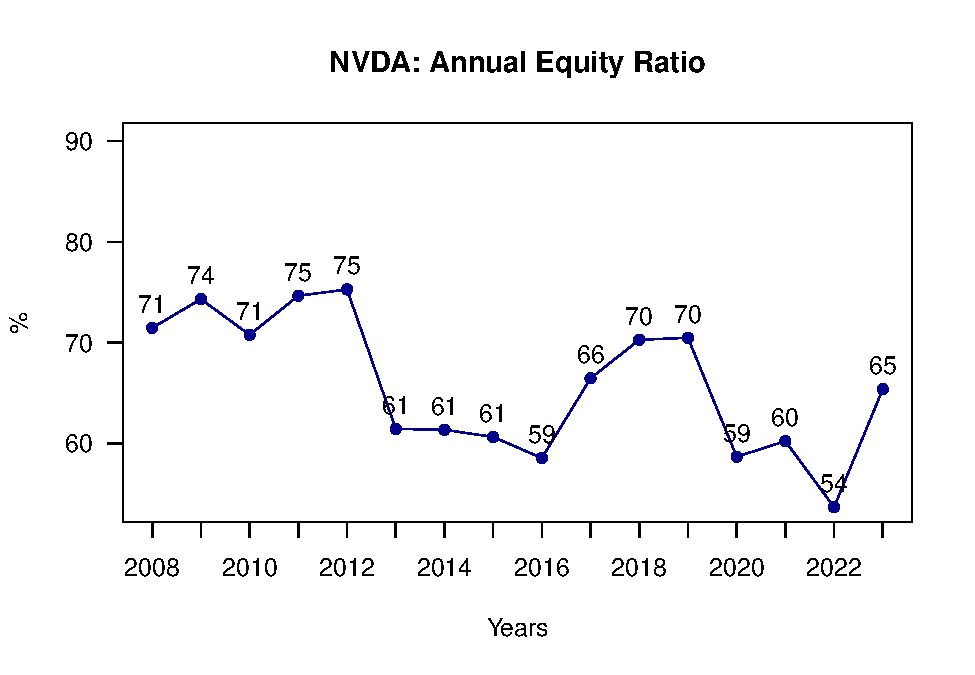
\includegraphics{_main_files/figure-latex/unnamed-chunk-1-4.pdf}
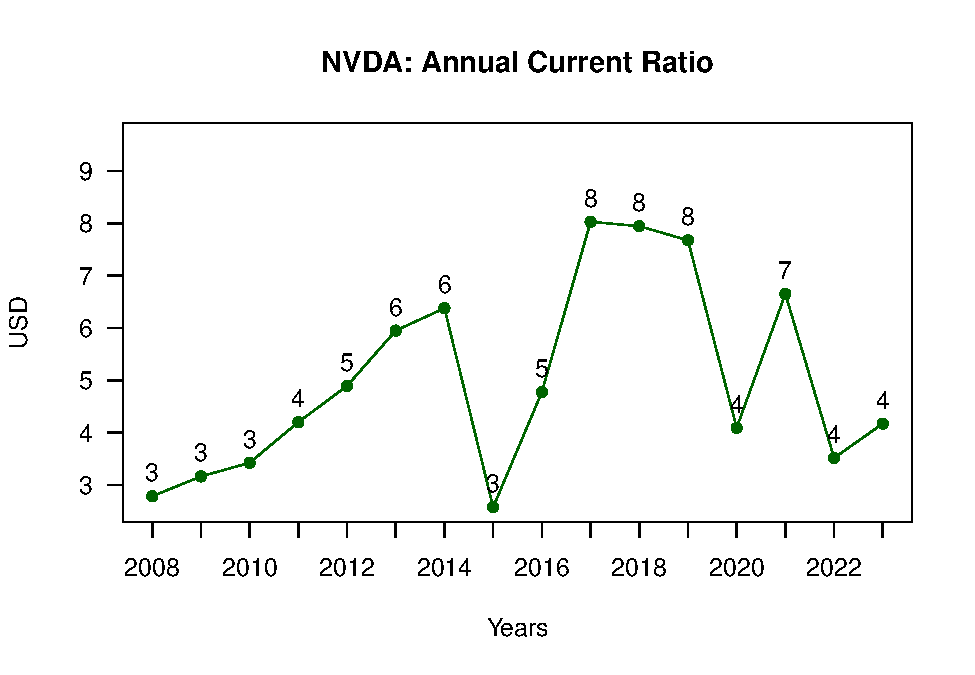
\includegraphics{_main_files/figure-latex/unnamed-chunk-1-5.pdf}

\hypertarget{smci}{%
\section{SMCI}\label{smci}}

Super Micro Computer Inc.~(SMCI): This American company manufactures computer servers, particularly high-performance and energy-efficient ones, for data centers, enterprise computing, and cloud computing .

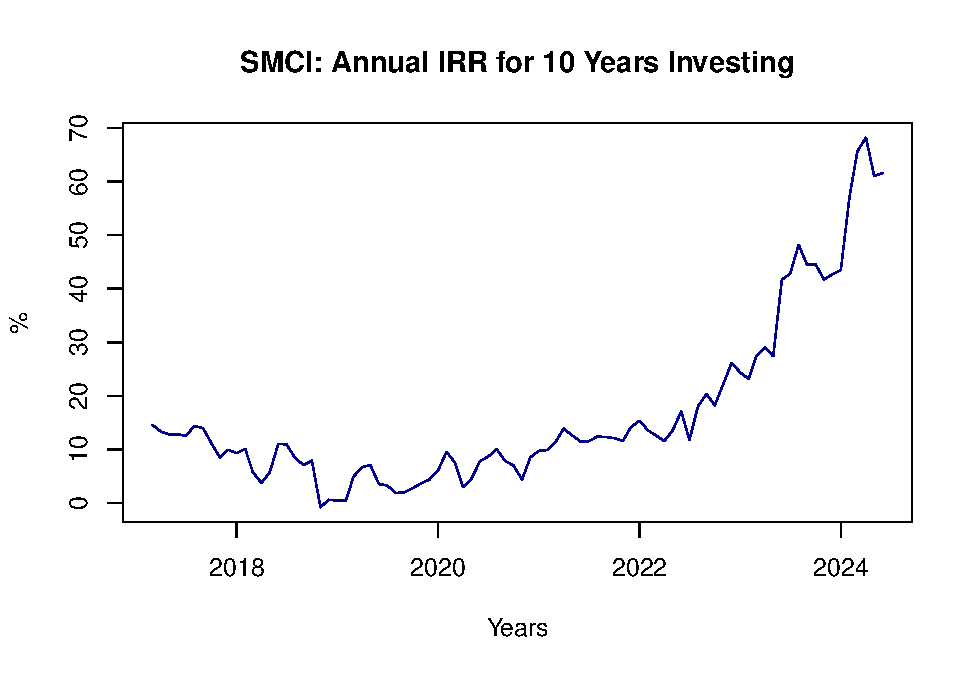
\includegraphics{_main_files/figure-latex/unnamed-chunk-1-6.pdf}
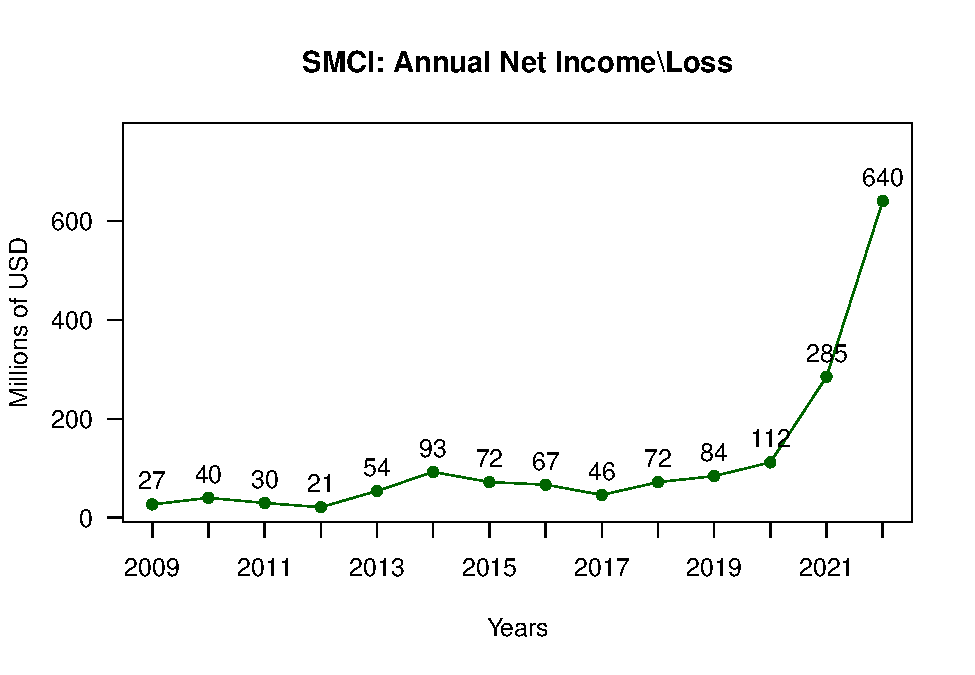
\includegraphics{_main_files/figure-latex/unnamed-chunk-1-7.pdf}
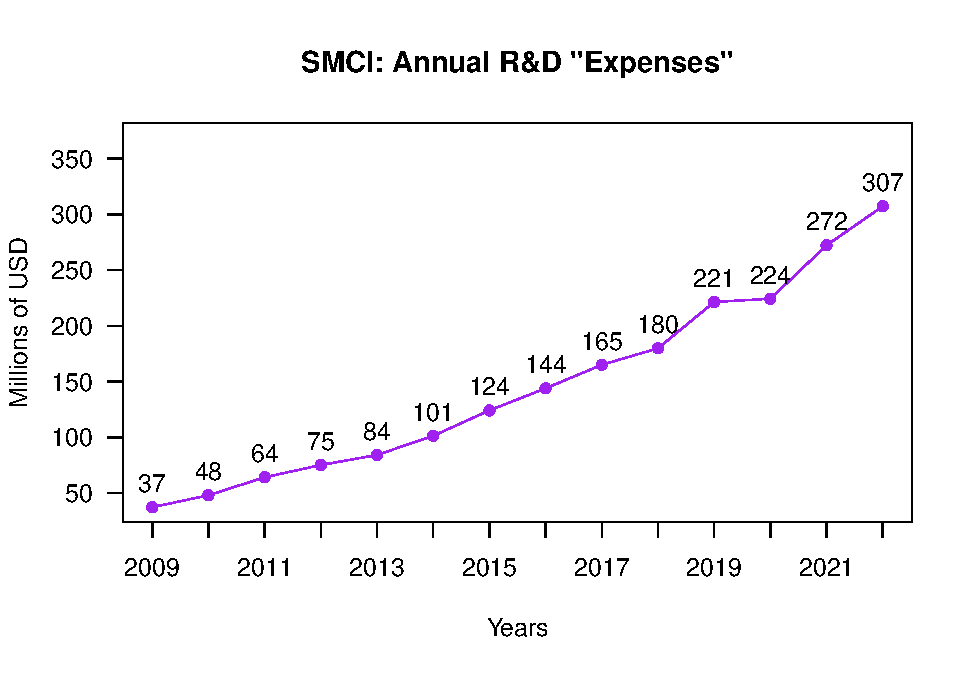
\includegraphics{_main_files/figure-latex/unnamed-chunk-1-8.pdf}
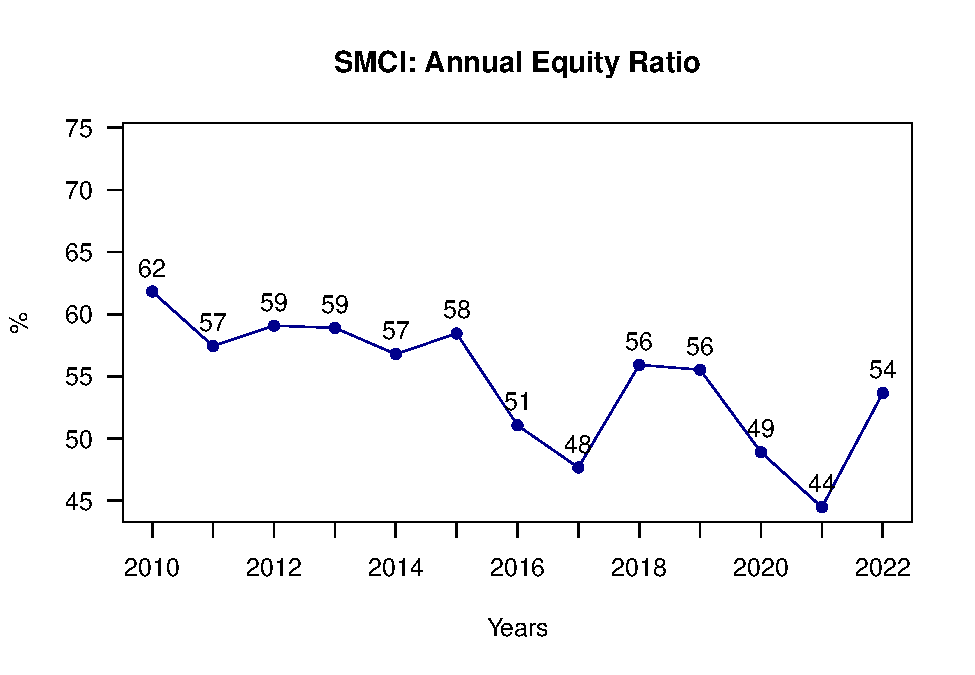
\includegraphics{_main_files/figure-latex/unnamed-chunk-1-9.pdf}
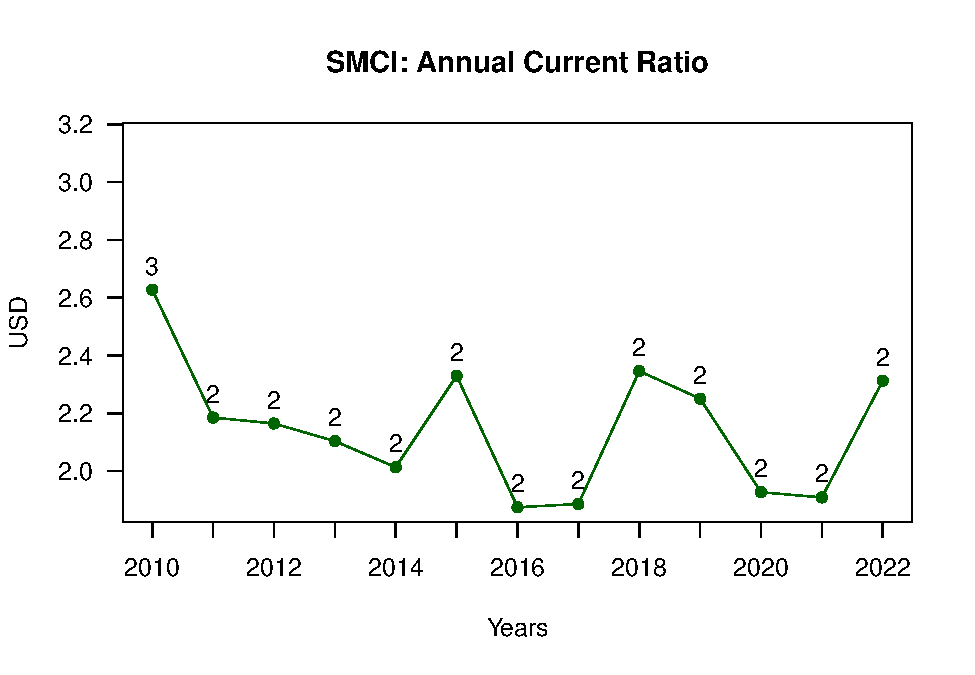
\includegraphics{_main_files/figure-latex/unnamed-chunk-1-10.pdf}

\hypertarget{zyxi}{%
\section{ZYXI}\label{zyxi}}

Zynex Medical Inc.~(ZYXI): This medical technology company develops and sells non-invasive monitoring and electrotherapy products used for sleep apnea, chronic pain management, and cardiac monitoring .

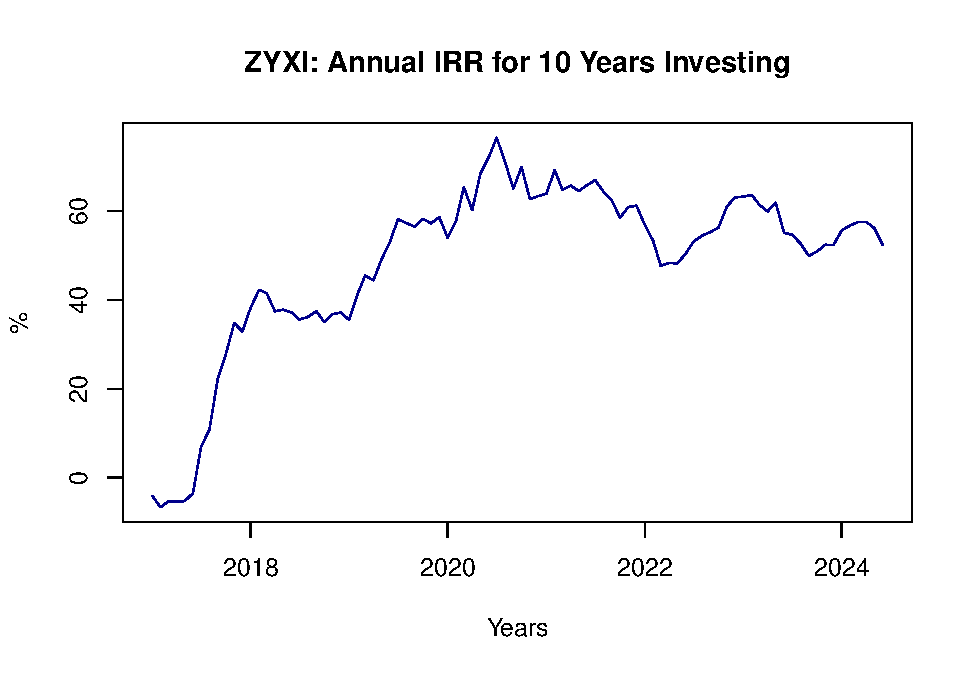
\includegraphics{_main_files/figure-latex/unnamed-chunk-1-11.pdf}
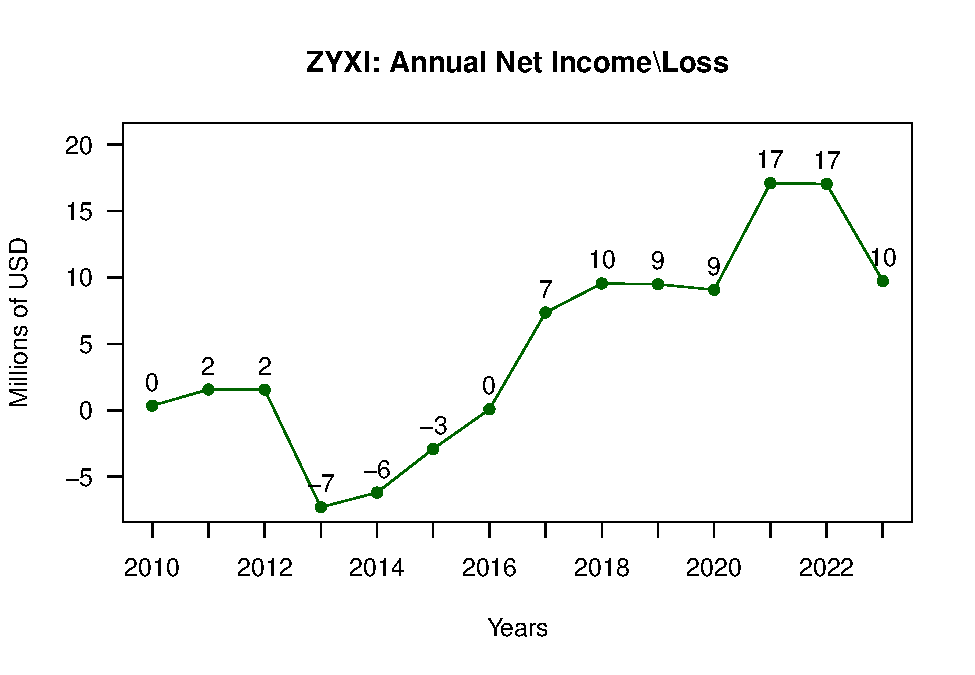
\includegraphics{_main_files/figure-latex/unnamed-chunk-1-12.pdf}
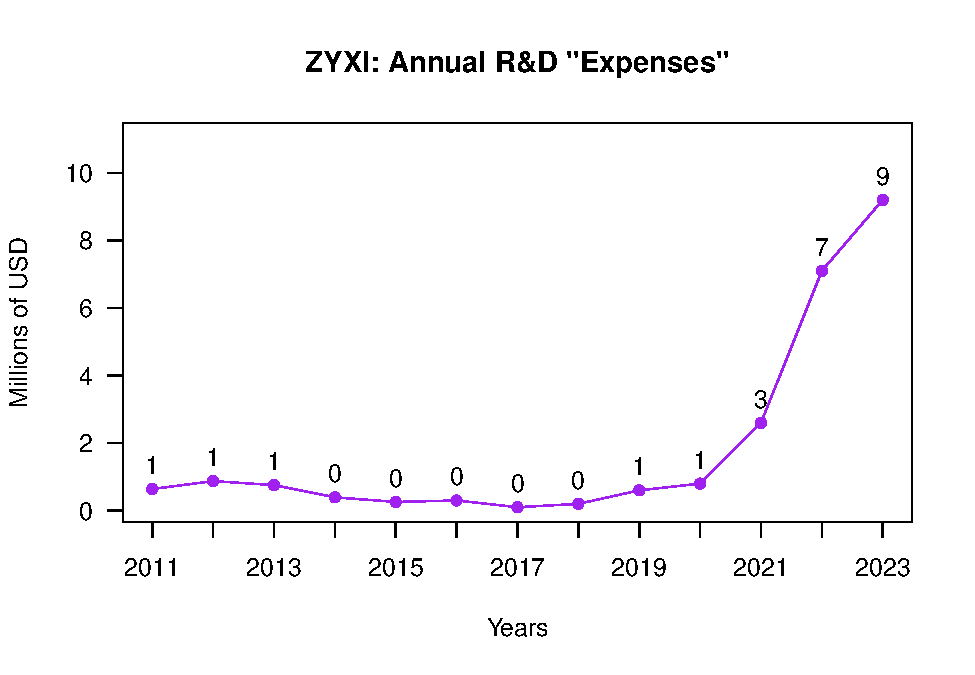
\includegraphics{_main_files/figure-latex/unnamed-chunk-1-13.pdf}
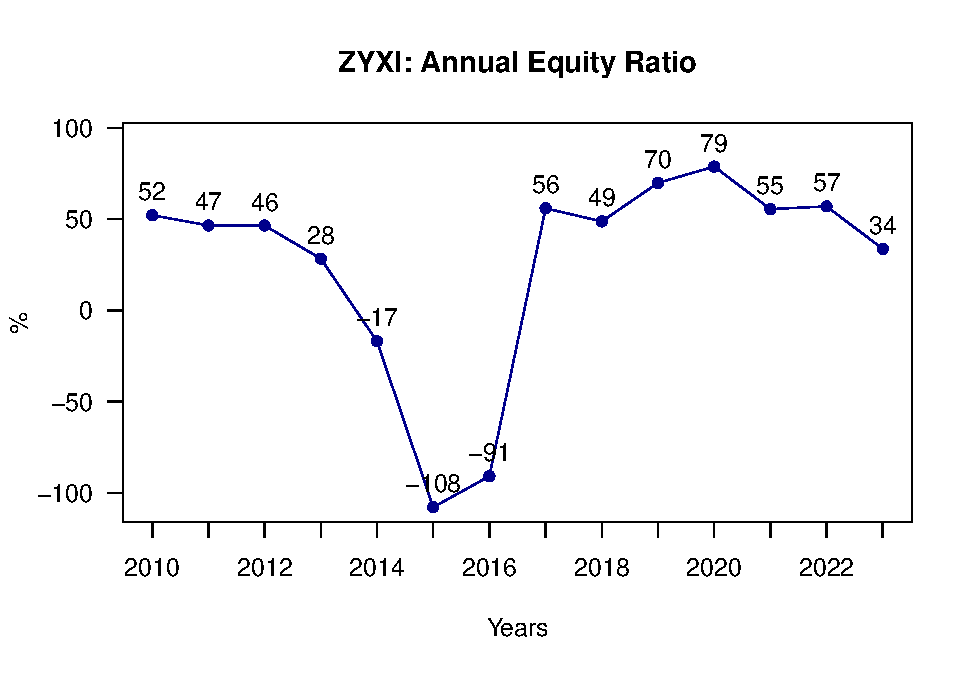
\includegraphics{_main_files/figure-latex/unnamed-chunk-1-14.pdf}
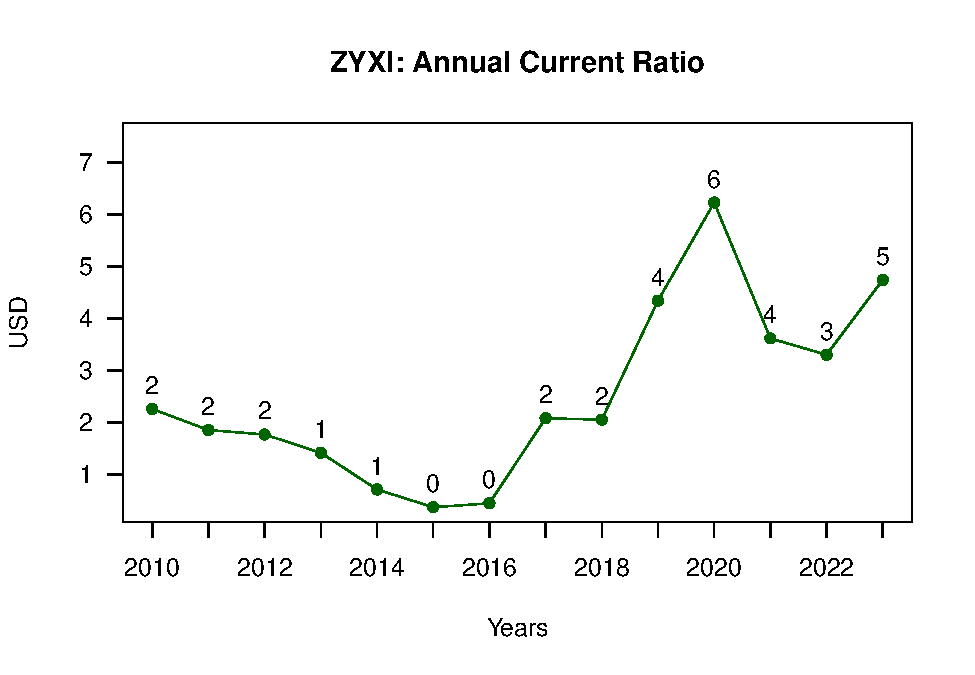
\includegraphics{_main_files/figure-latex/unnamed-chunk-1-15.pdf}

\hypertarget{lrcx}{%
\section{LRCX}\label{lrcx}}

Lam Research Corporation (LRCX): This company supplies equipment used in the semiconductor manufacturing process. Their equipment etches patterns onto silicon wafers, a crucial step in creating computer chips .

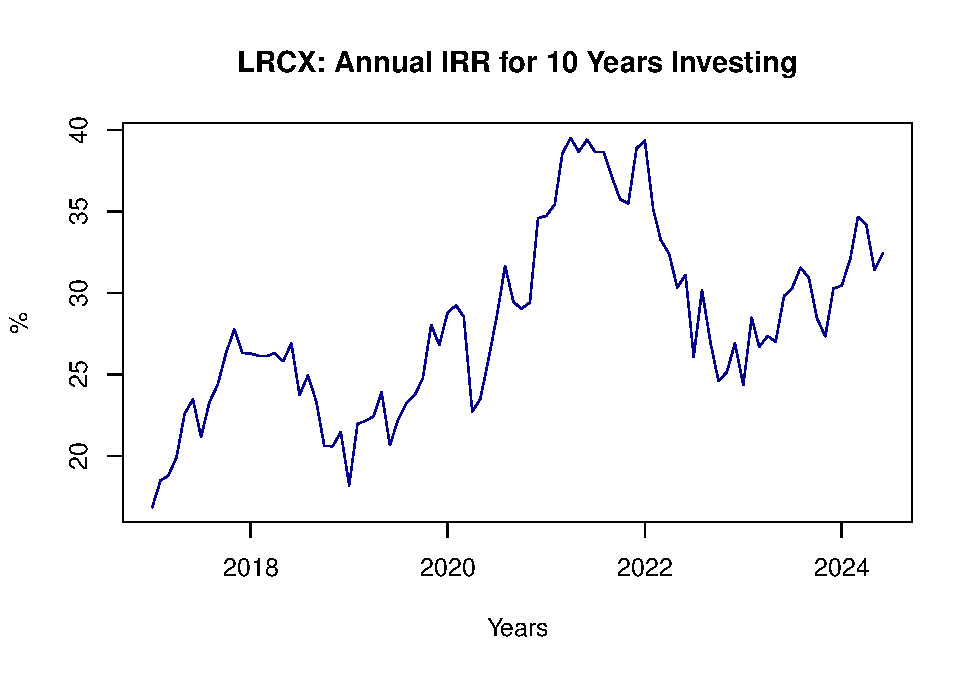
\includegraphics{_main_files/figure-latex/unnamed-chunk-1-16.pdf}
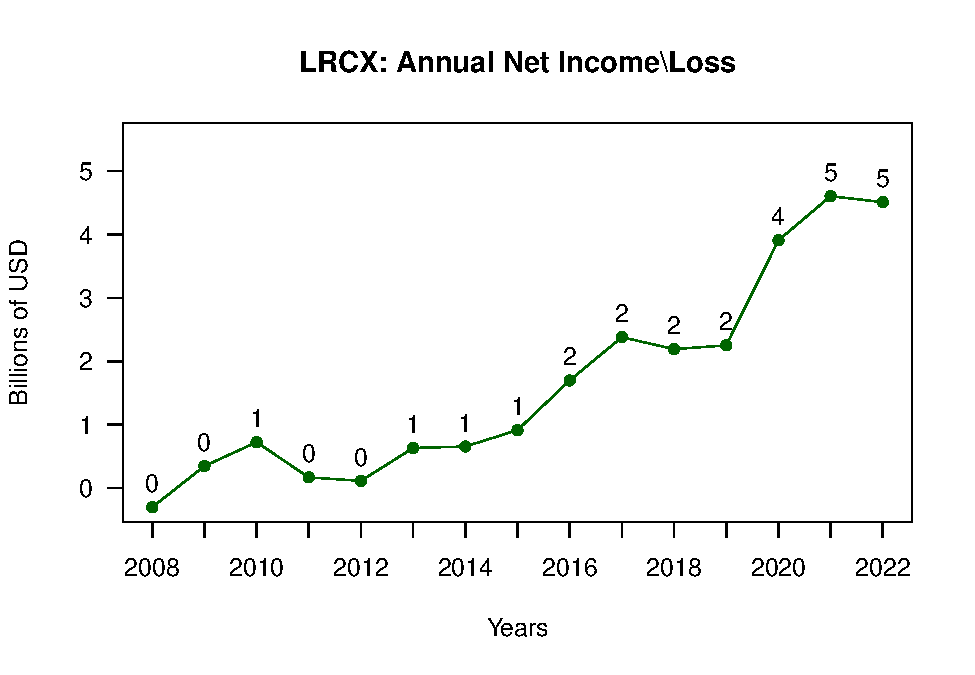
\includegraphics{_main_files/figure-latex/unnamed-chunk-1-17.pdf}
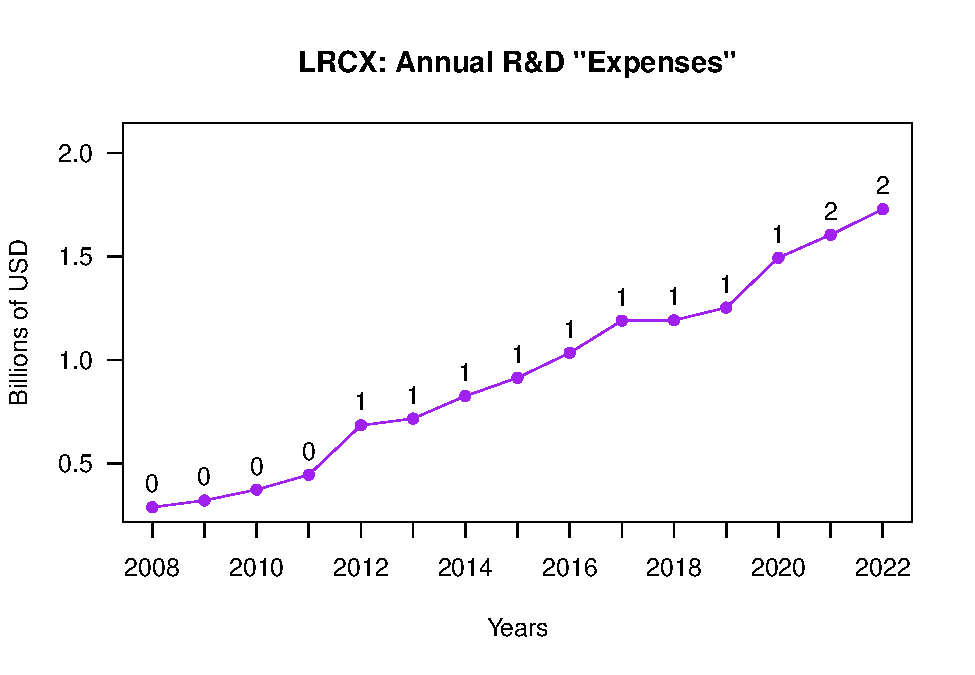
\includegraphics{_main_files/figure-latex/unnamed-chunk-1-18.pdf}
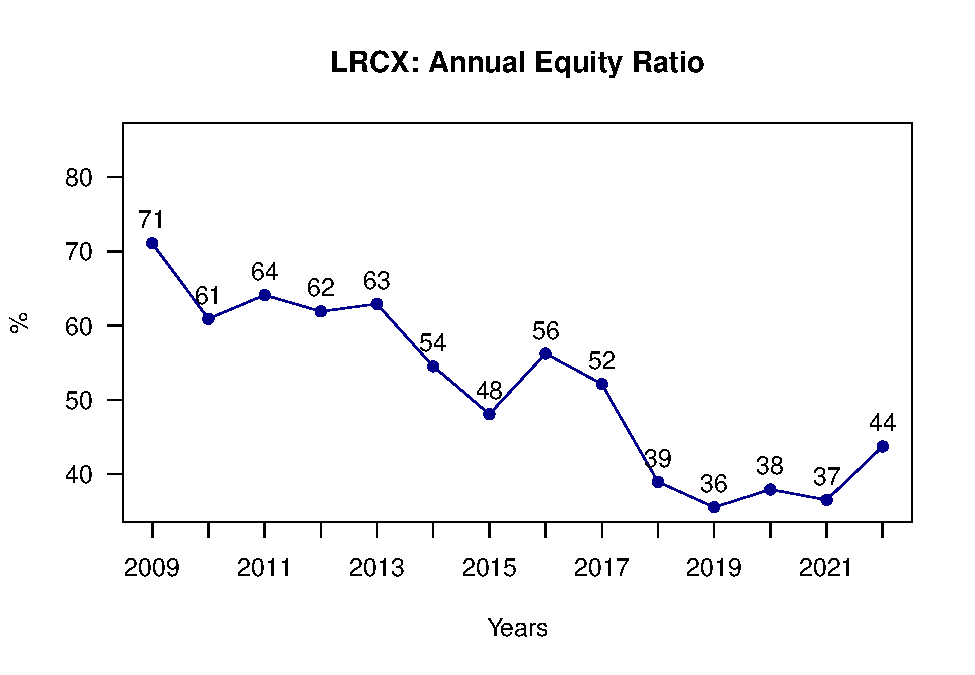
\includegraphics{_main_files/figure-latex/unnamed-chunk-1-19.pdf}
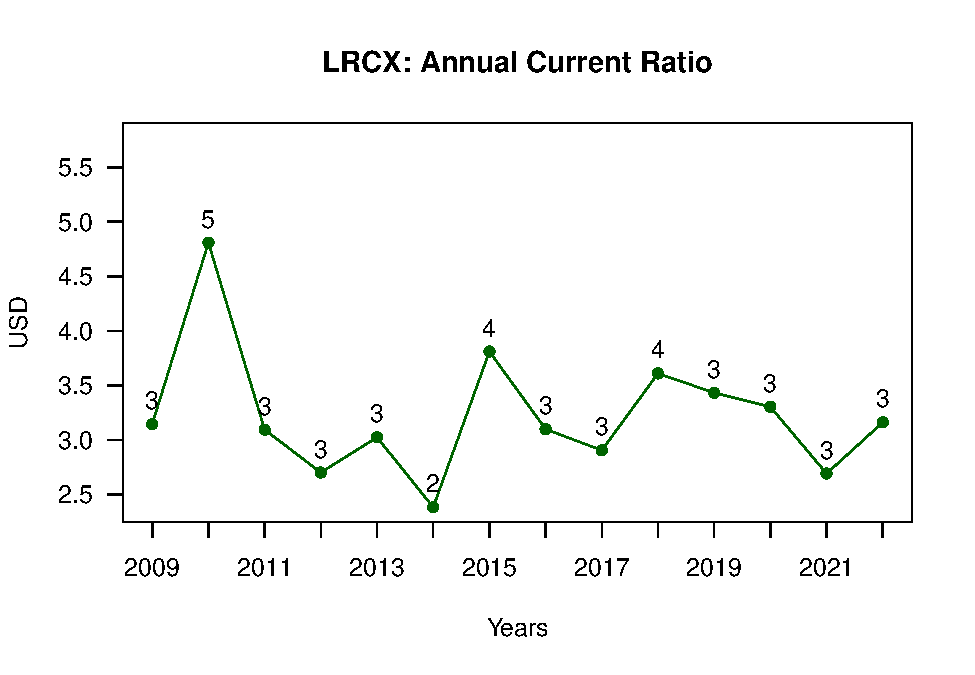
\includegraphics{_main_files/figure-latex/unnamed-chunk-1-20.pdf}

\hypertarget{googl}{%
\section{GOOGL}\label{googl}}

Alphabet Inc.~(GOOGL): This is the parent company of Google and several other subsidiaries like YouTube and Fitbit. They specialize in internet-related services and products, including search engines, online advertising, cloud computing, and software .

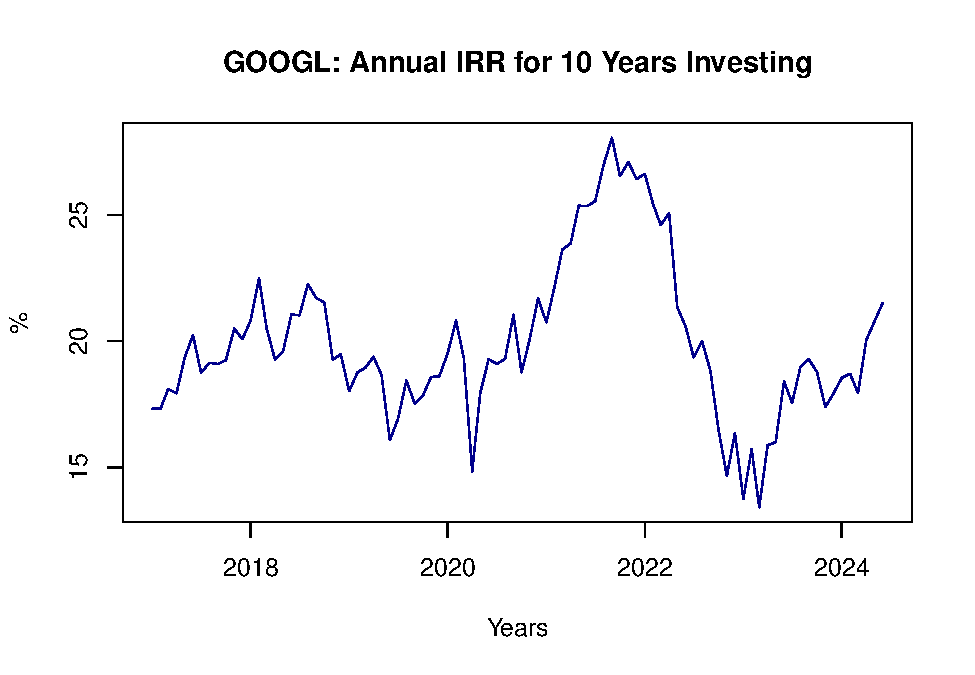
\includegraphics{_main_files/figure-latex/unnamed-chunk-1-21.pdf}
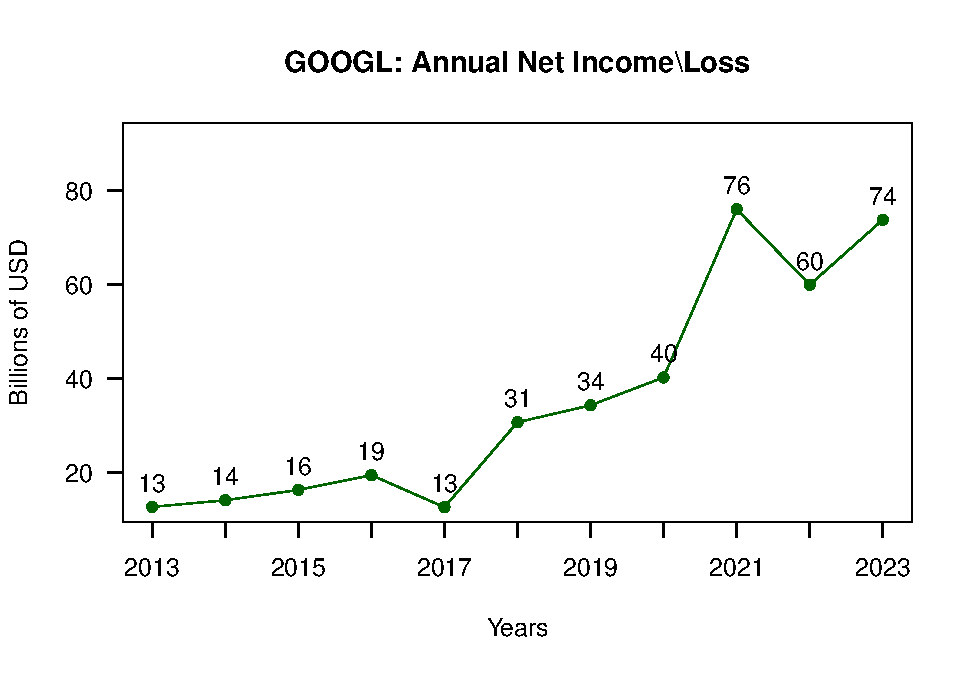
\includegraphics{_main_files/figure-latex/unnamed-chunk-1-22.pdf}
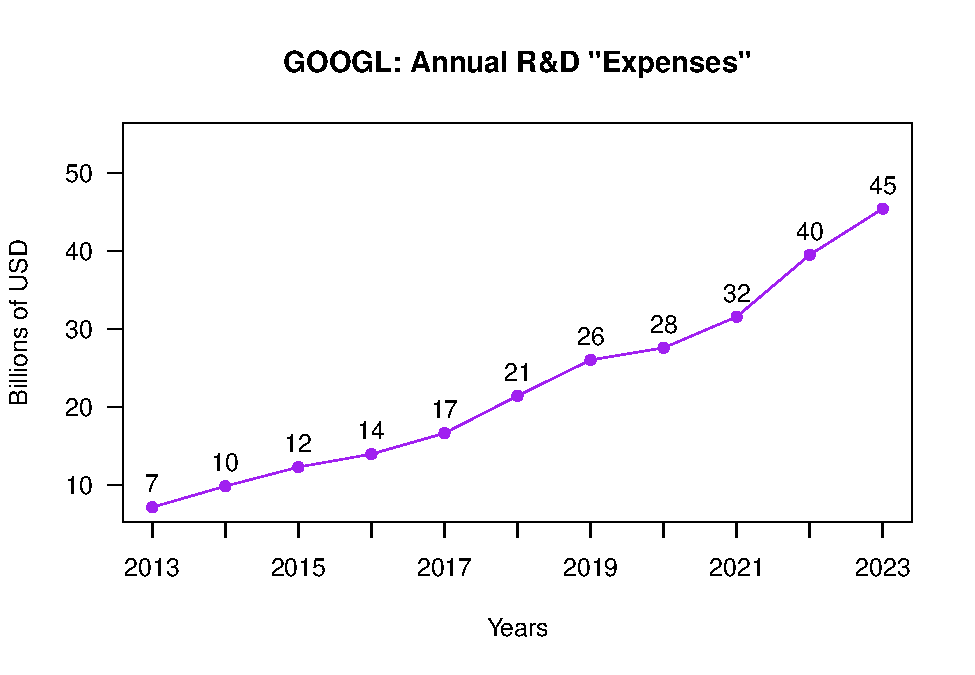
\includegraphics{_main_files/figure-latex/unnamed-chunk-1-23.pdf}
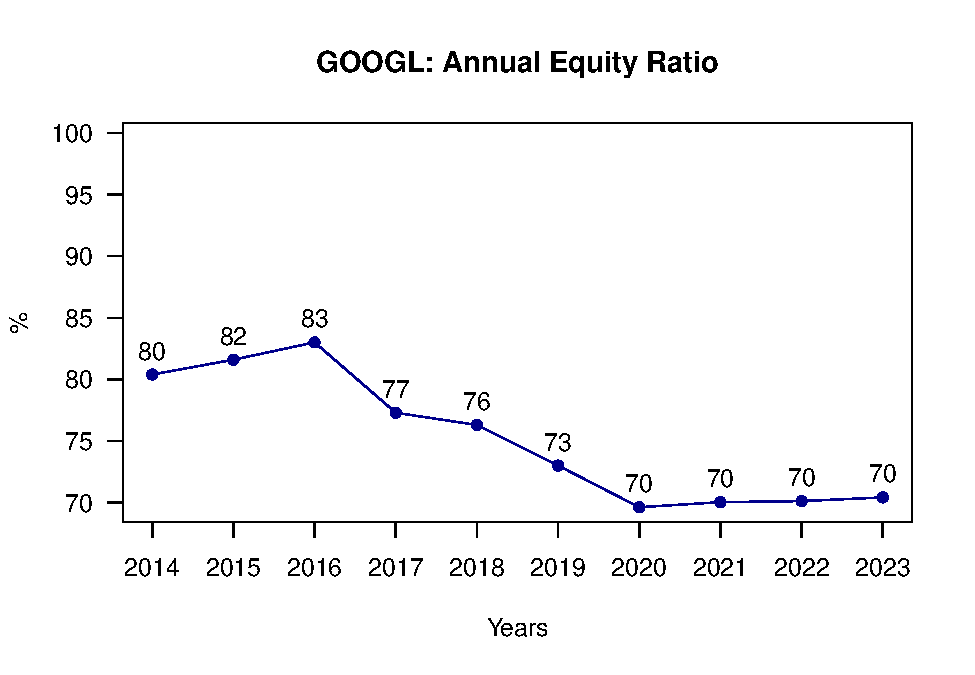
\includegraphics{_main_files/figure-latex/unnamed-chunk-1-24.pdf}
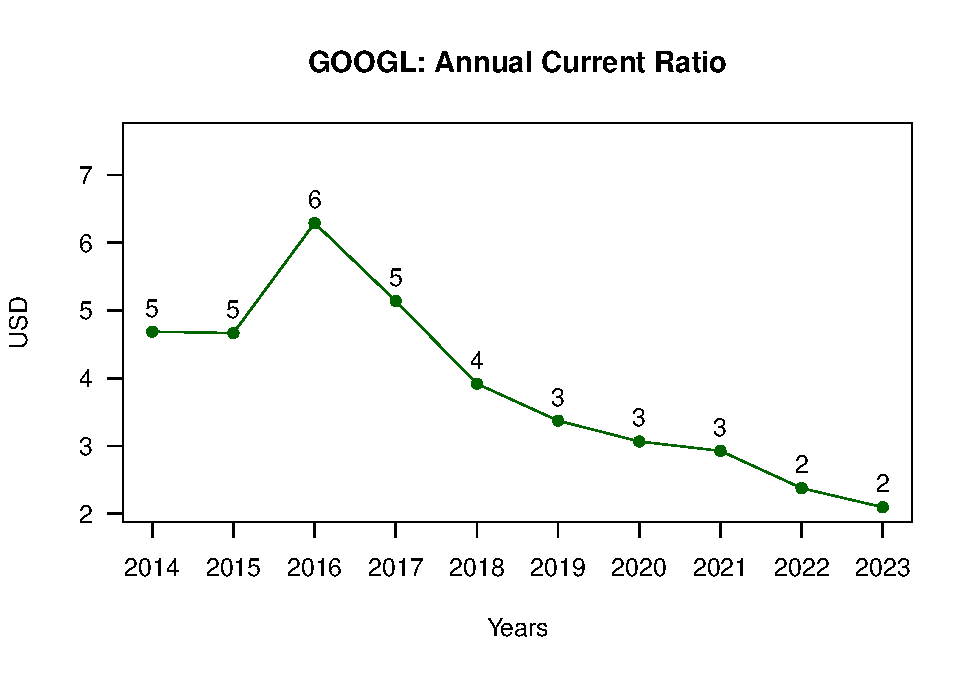
\includegraphics{_main_files/figure-latex/unnamed-chunk-1-25.pdf}

\hypertarget{intu}{%
\section{INTU}\label{intu}}

Intuit Inc.~(INTU): This company develops financial software, most well-known for their tax preparation software TurboTax and personal finance app Mint .

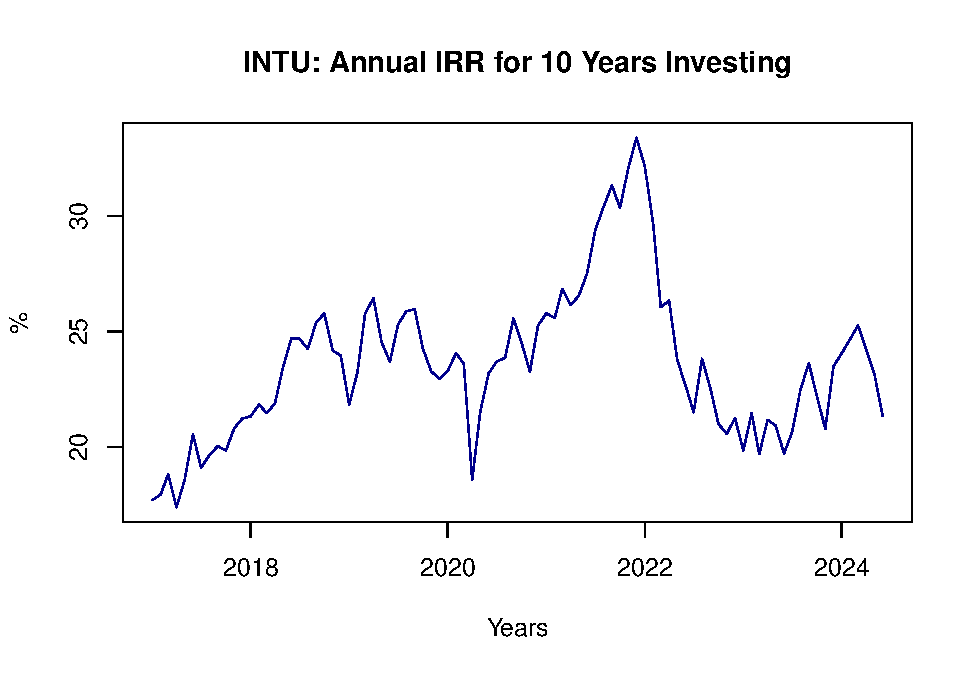
\includegraphics{_main_files/figure-latex/unnamed-chunk-1-26.pdf}
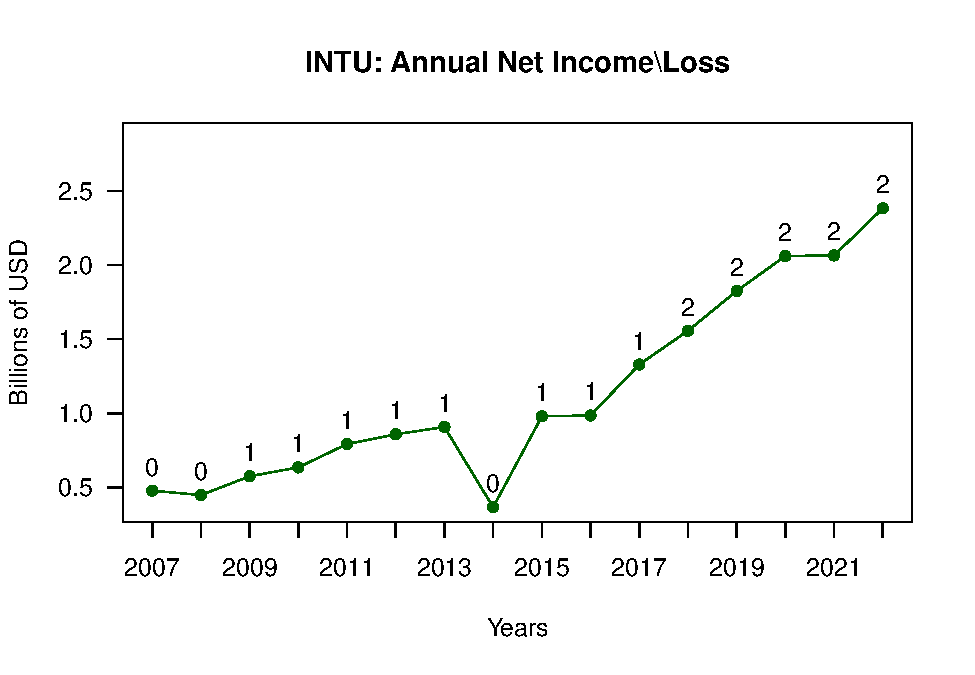
\includegraphics{_main_files/figure-latex/unnamed-chunk-1-27.pdf}
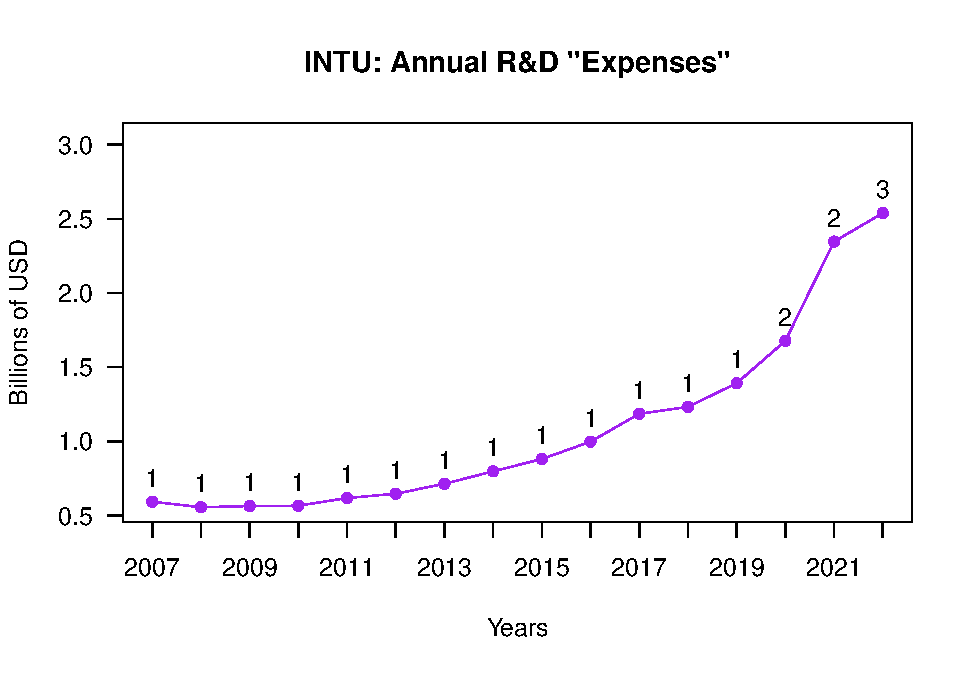
\includegraphics{_main_files/figure-latex/unnamed-chunk-1-28.pdf}
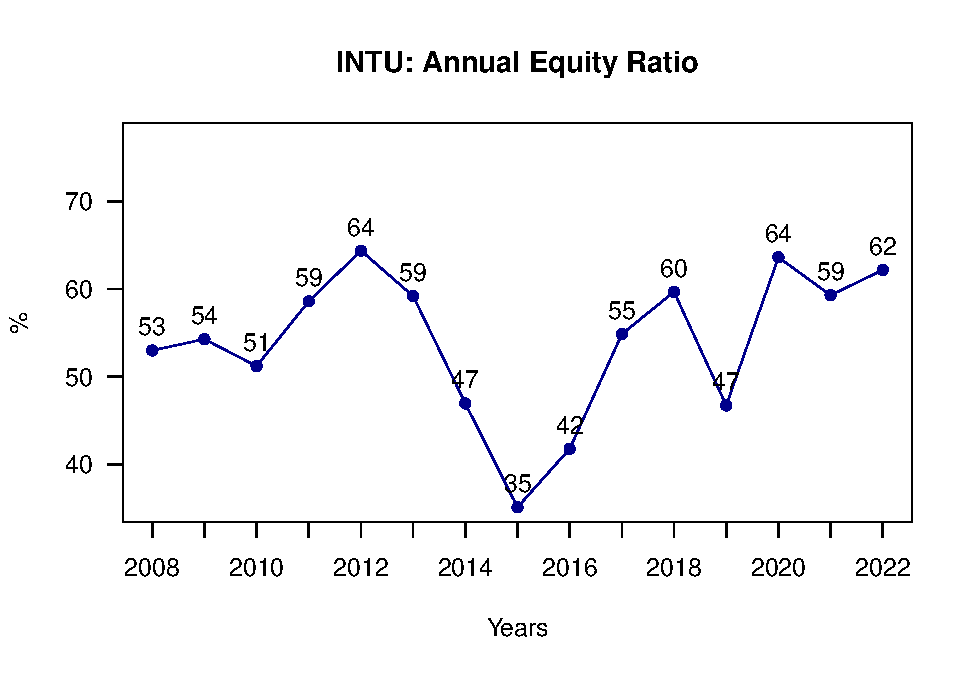
\includegraphics{_main_files/figure-latex/unnamed-chunk-1-29.pdf}
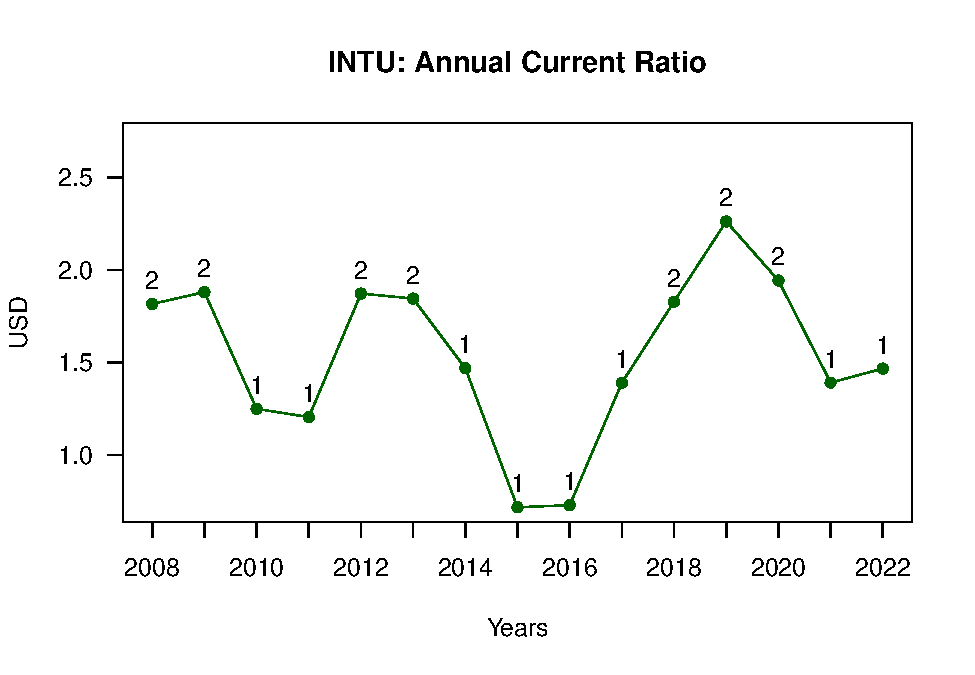
\includegraphics{_main_files/figure-latex/unnamed-chunk-1-30.pdf}

\hypertarget{irr-rank}{%
\chapter{IRR Rank}\label{irr-rank}}

\begin{tabular}{l|l|r}
\hline
Ticker & Company & Actual IRR (\%)\\
\hline
NVDA & NVIDIA CORP & 77.76\\
\hline
SMCI & Super Micro Computer, Inc. & 61.61\\
\hline
ZYXI & ZYNEX INC & 52.41\\
\hline
LRCX & LAM RESEARCH CORP & 32.47\\
\hline
GOOGL & Alphabet Inc. & 21.49\\
\hline
INTU & INTUIT INC. & 21.34\\
\hline
\end{tabular}

\end{document}
